
\documentclass[a4paper,11pt]{article}
% define the title
\usepackage{graphicx}
\usepackage{hyperref}
\author{GDP Group 18}
\title{UAV Image Viewer User Guide}
\begin{document}
% generates the title
\maketitle
%\newpage
% insert the table of contents
%\tableofcontents
%\newpage
\section{Before Starting the UAV Image Viewer Program}
\label{sec:initial}
In order to connect the payload and camera to the UAV,
the user needs to connect an ethernet cable between the Autopilot and Payload modules.
The Autopilot powers the payload module, as well as providing a medium for the 
two modules to communicate.
The user should not have to connect the camera manually as it should already be connected. 

\begin{figure}[!htbp]
\label{fig:payload}
\begin{center}
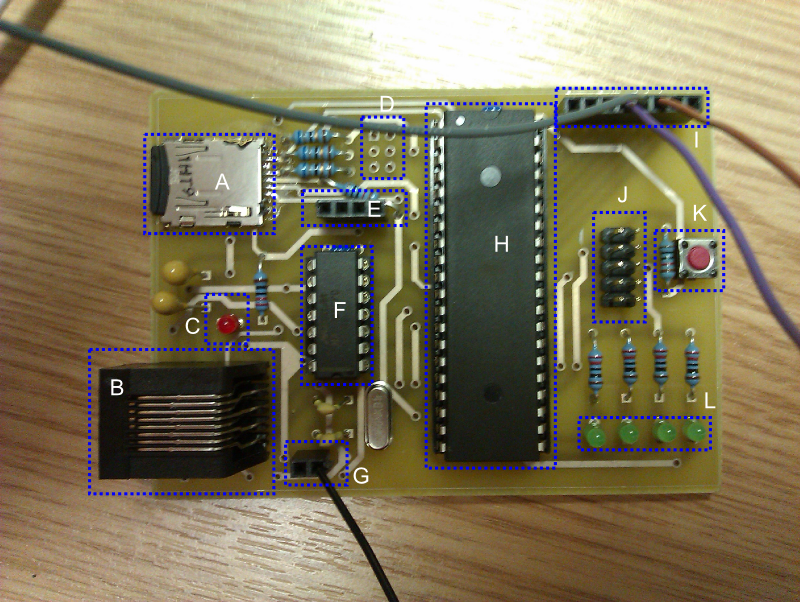
\includegraphics[width=0.8\textwidth]{PayloadImplementation.png} 
\caption{The Payload Module}
\end{center}
\end{figure}

Please check the following features on the payload once it has been connected 
to the Autopilot and the Autopilot is powered:

\begin{itemize}
	\item The Power LED (C) should be lit.
	\item A microSD card should be present in socket (A). It is preferred if 
this card is SDSC and not SDHC or SDXC standard. Please make sure this card 
has enough memory to take the images.
	\item Images stored locally are up to approximately 30kB in size, and 
are stored in the filename test\$NUMBER.jpg (replace \$NUMBER with an integer between 0 and 32768)
	\item If you are using more payload modules than this, and they are 
sourcing more than 150mA from the Autopilot, please power this payload module 
externally. On Header G, connect 3.3V to the left-hand, and GND to the 
right-hand socket.
	\item (K) is a reset button. 
	\item In case the camera is disconnected, from L-R on (E), are 3.3V, 
GND, Camera TX and Camera RX. Please refer to the Camera Schematics. \footnote{\url{http://www.4dsystems.com.au/downloads/micro-CAM/Docs/uCAM-DS-rev4.pdf}}
\end{itemize}

Full schematics, PCB layout and Gerber Files are available in our official GitHub repository \footnote{\url{https://github.com/uavcamera/uavcamera}}, 
in the schematics/ file.

On the ground side, the Autopilot's receiver module needs to be connected to a USB socket.
Figure \ref{clipArt} shows the diagram of how to connect the payload to the UAV and the UAV data receiver to the computer. 

\begin{figure}[!htbp]
\begin{center}
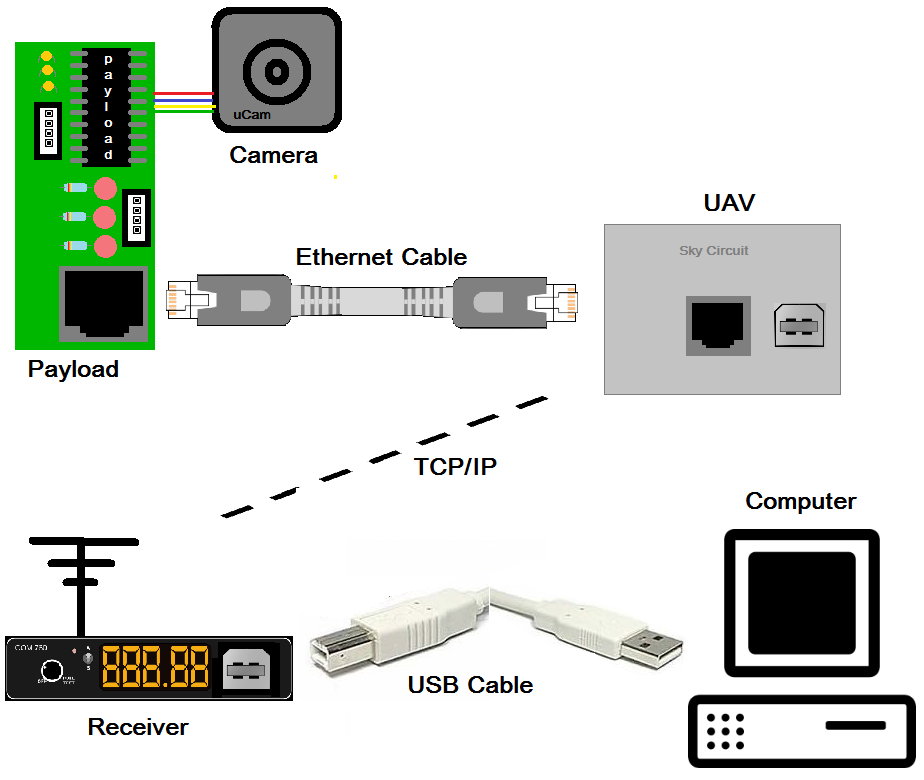
\includegraphics[width=0.8\textwidth]{clipArt.png} 
\caption{The Clip Art of the Hardware Connection Diagram \label{clipArt}}
\end{center}
\end{figure}

For the UAV Image Viewer to work correctly, the receiver must first be connected to the ground station. 
In order to connect to the receiver, all the hardware has to be connected as described above.
The GCS station then connects to the Autopilot receiver by clicking on the Connect button. If the program does not connect to the Autopilot automatically, the user can select it from the combo box. Then check the "Enable Network Server" box. Figure \ref{GCS} shows a screen shot of the GCS program.
If the autopilot does not appear, the user should check the connection of the UAV and make sure that the driver of the USB has already installed. 

To install the USB driver:

 Run "Device Manager" $\rightarrow$ Right click on the UAV $\rightarrow$ Click on the update driver$\rightarrow$ Find the driver (.inf file) $\rightarrow$ install it $\rightarrow$ UAV is ready to use.

\begin{figure}[!htbp]
\begin{center}
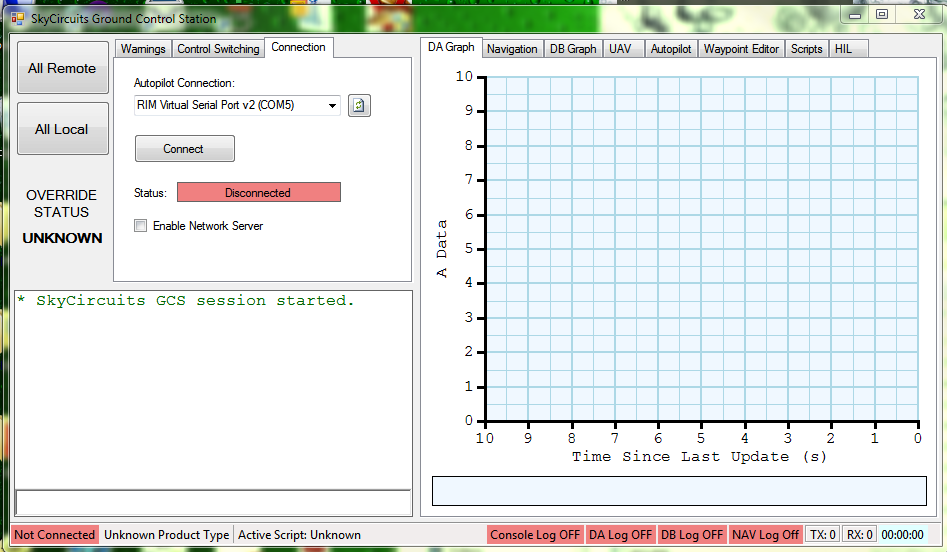
\includegraphics[width=0.5\textwidth]{GCS.PNG}  
\caption{The Ground Control Station Software \label{GCS}}
\end{center}
\end{figure}
 


\section{UAV Image Viewer Ground Station}

\begin{figure}[!htbp]
\begin{center}
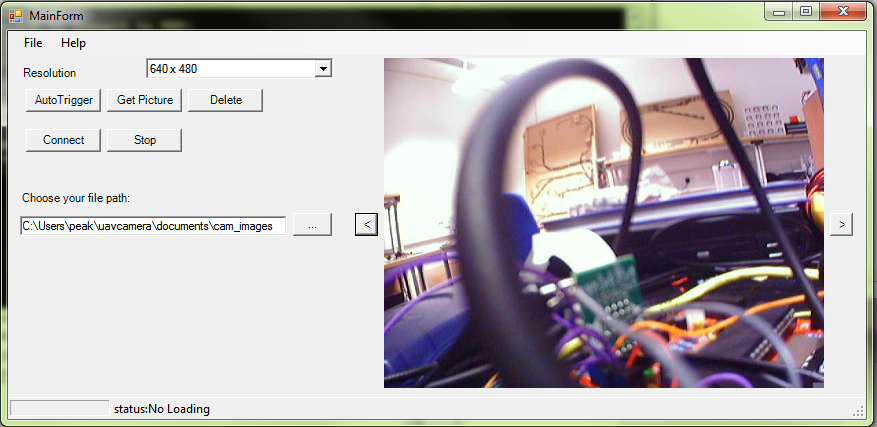
\includegraphics[width=0.8\textwidth]{windowApplication.PNG}  
\caption{The UAV Image Viewer Software\label{IVP}}
\end{center}
\end{figure}

The file tab in the top left corner allows the user to open a file, then display it in the picture box, and save this image to a specified directory. It also gives the option to exit the program. Figure \ref{openTab} shows the diagram of the file tab.

\begin{figure}[!htbp]
\begin{center}
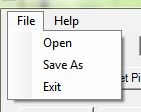
\includegraphics[width=1.0\textwidth]{FileButton.png}  
\caption{Open Tab \label{openTab}}
\end{center}
\end{figure}

The user can choose the resolution from the drop-down menu in the top left. There are four options - all of the resolutions that the camera can take. The lower the resolution, the quicker the image downloads. 

\begin{figure}[!htbp]
\begin{center}
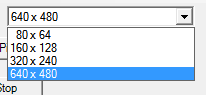
\includegraphics[width=1.0\textwidth]{comboBoxResolution.png}   
\caption{The Resolution Option \label{resOp}}
\end{center}
\end{figure}

Figure\ref{buttons} shows some buttons present in our application. The \textbf{AutoTrigger} button allows the user to take multiple photos and save them on the on-board microSD card. The \textbf{Get Picture} button will allow the user to take a picture and send it directly to the ground station. The default file name of the picture will be uavPictureAtyyyy-MM-dd\_hh-mm-ss-tt.jpg. The photo will be saved in the file path specified in the text box as shown in figure \ref{filePath}. The name depends on the system date and time at the time of taking picture. It will take about 10-20 seconds from clicking "Get Picture" to displaying the image.

\begin{figure}[!htbp]
\begin{center}
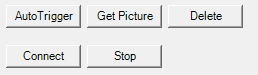
\includegraphics[width=1.0\textwidth]{button.PNG}  
\caption{The Buttons Options of the Image Picture Viewer\label{buttons}}
\end{center}
\end{figure}

\begin{figure}[!htbp]
\begin{center}
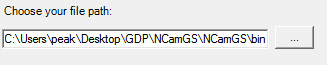
\includegraphics[width=1.0\textwidth]{filePath.PNG} 
\caption{The file path text box\label{filePath}}
\end{center}
\end{figure}

The left and right buttons near the picture allow the user to change the photo displayed to any locally stored jpeg image in the selected file path. The button is shown in figure \ref{leftRight}. 

\begin{figure}[!htbp]
\begin{center}
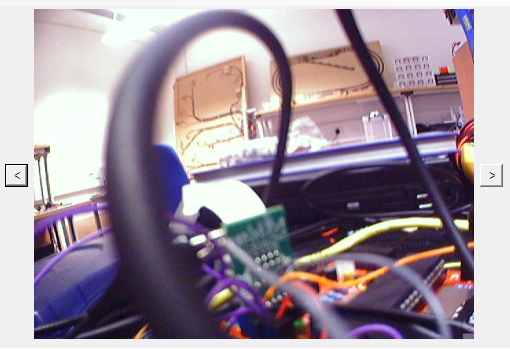
\includegraphics[scale=1]{leftRight.PNG}   
\caption{The Picture Box with left and right buttons \label{leftRight}}
\end{center}
\end{figure}

The progress bar shows the proportion of the image that has arrived at the ground station. The status label will tell what signal is send and receiving so the user can keep track of what is going on in the payload.

\begin{figure}[!htbp]
\begin{center}

\includegraphics[scale=1]{progress_bar.PNG} 
\caption{The progress bar and the status text \label{progressBar}}
\end{center}
\end{figure}

\subsection{Take Picture}

The use can simply click on the Get Picture button in the program. Figure \ref{buttons} shows where the button is.

\end{document}
